	\section{Overall Description}
		\subsection{Product Perspective}
	      Tickets Tonight is a follow-on member of Ticketmaster’s mobile app for ticket sales. Ticket Tonight 
	      will be focused and catered to users making last minute decisions to go to an event. Tickets Tonight 
	      will use the event, artist, category, venue, and affinity data provided by Ticketmaster to achieve its 
	      purpose. The data given by Ticketmaster will allow the Tickets Tonight to provide the user actual 
	      events that they may be interested in. If Ticketmaster desires, this application could be integrated with 
	      their actual database instead of pre-generated data. In order to better cater to the user, the application 
	      will use the user’s favorite artists to generate more relevant recommendations of events. Ticketmaster 
	      could later link their user database to this application but without any given API, this version of 
	      Tickets Tonight will generate its own user group separate from Ticketmaster users. Tickets Tonight’s 
	      user data and favorite artists will be stored on Parse. For preliminary and testing purposes, the 
	      application will use anonymous users and will not store actual user favorites. 
		\begin{center}
			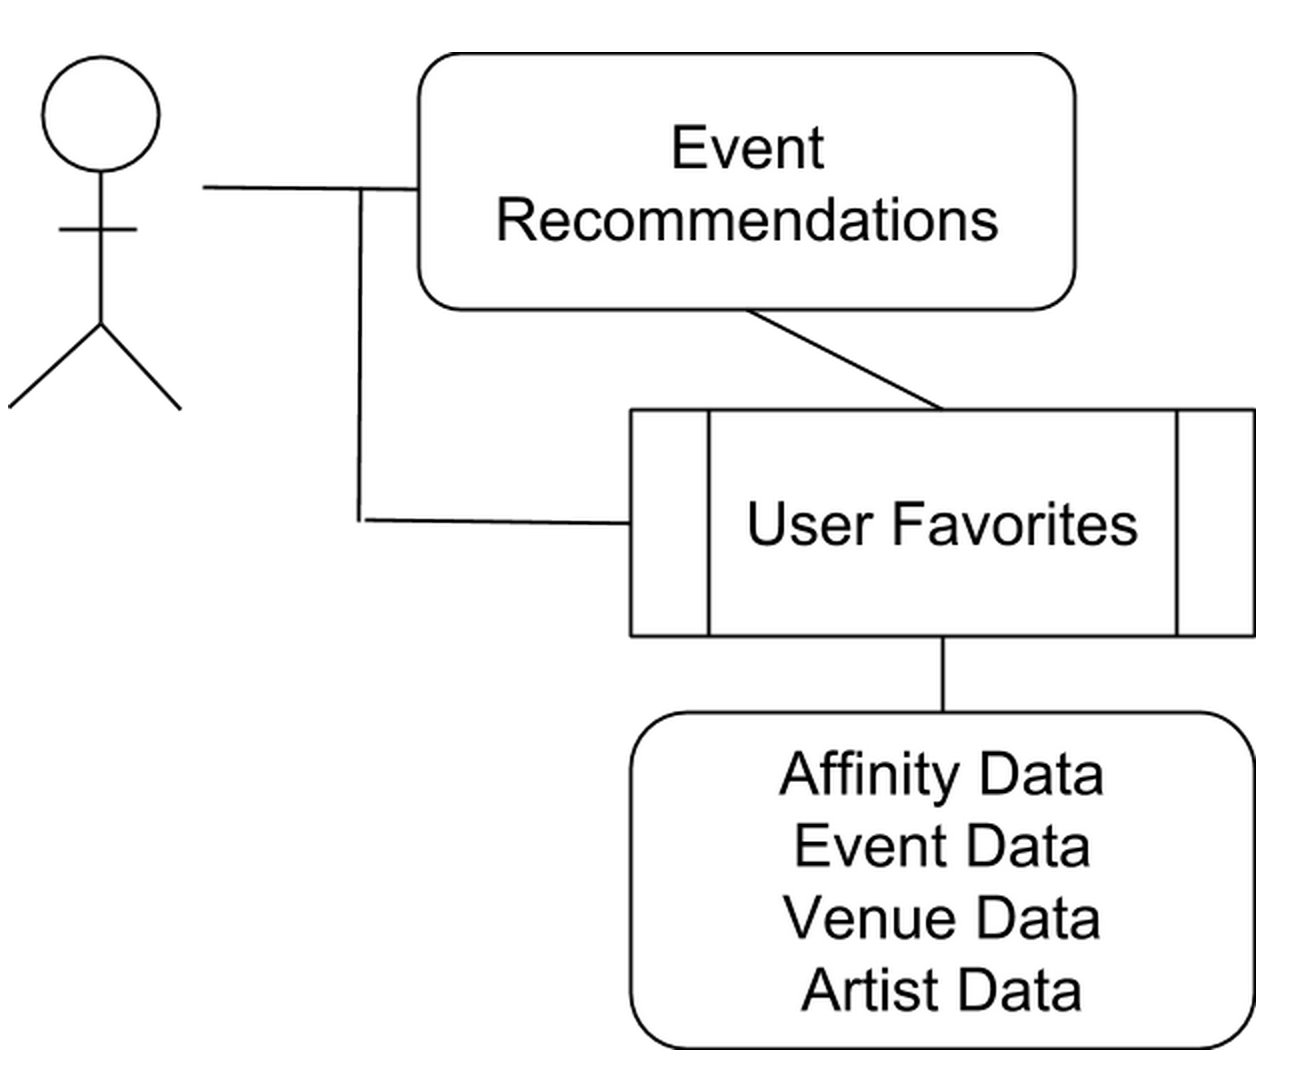
\includegraphics[width=90mm]{./pics/pp1.png}
			\captionof{figure}{Product perspective}
		\end{center}
		\subsection{Production Features}
		 The overall application will have a Feed view, a Favorites view, a Explore view and a Settings(More) view. 
	 	 More details of the following views will be provided in Section 3. The following descriptions provide a 
		 high level summary. Each of the following views will be a view inside a UI tab bar controller object in the app. 
		 The views will be accessible through tabs on the bottom.
		
		 Feed View: In this view, the user would be able to see the events of their favorite artists and the events 
		 will be ordered by date. This view will be separated into recent, favorite and following tabs. The recent 
		 tab of the feed view will display the events that are happening near the user (if location turned on) and 
		 events will be sorted by date. The favorite tab in the feed view allows the user to view his or her 
		 favorited artists’ recent events. In addition, there is also the following tab which allows the user to 
		 easily track the events that he or she has followed. The events that the user has followed could be 
		 events he or she is going or simply the user just wants to track it. Furthermore, if the event that the 
		 user is following changes location, the user can easily track that change and get notified.
		
		 Favorites view: In this view, the user would be able to see the artists they have selected as their favorite 
		 artists. The user would be able to click on any of the artist cells and untoggle the favorite selection if 
		 he or she so desires. At the top of this view the user can also manually search for artists by their names 
		 to find the artist the user wants to add and start tracking. The search will research and refine the results 
		 as the user types in letters. For each key stroke we can further reduce the result pool and create a 
		 almost search-auto complete feature.
		
		 Explore view: In this view, the user will be provided a slide card presentation of potential events that 
		 the user may be interested in. The user can slide away the cards if the user is not interested. The events 
		 presented in this view is generated through the affinity data by first joining the lists of artists that are 
		 similar to the user’s favorite artists, then finding events performed by those related/similar artists. If 
		 the user does not have a lot of favorite artists, the slide cards could eventually be emptied since the 
		 given data from Ticketmaster is not as expansive as their actual database. In the case where the cards 
		 are all swept out, there is a refresh button on top for the user to reset.
		
		 Settings view: In this view, the user will be able to search artists by category, toggle location control 
		 and a logout button. The logout button currently does not implement actual logging out or logging in 
		 action since this application will be using anonymous users hence the user favorite data will be stored 
		 locally on the phone. There is also another tab to allow the user to access the events nearby directly 
		 listing out all events nearby.
		
		\subsection{User Classes and Characteristics}
		  Currently the main type of user will be potential ticket buyers. They will be notified when an event 
		  would be a good match for them based on their favorite artists and affinity data. The main user base 
		  will likely be users who intend on going to events last minute and have not made plans. These types of 
		  users are typically whimsical or perhaps are from out of town. This user class could potentially also be 
		  people who had plans cancelled and need to kill time. They would benefit from the explore view that 
		  generates events of artists relatable to their favorite artists based on the affinity data. These are our 
		  favored user class. Another user class could be event planners that are planning an event for their 
		  customer and intend on avoiding conflicts with other popular events or other similar artists’ events. In 
		  other words, these users use the application to find out openings and times that they could host their 
		  own events without coming into conflicting with other events. These users are not the primary users 
		  that Tickets Tonight want to satisfy as they will not likely be purchasing tickets from Ticketmaster.

		 \subsection{Operating Environment}
		  Initially, the Tickets Tonight app will be built for Apple’s iOS 8 mobile operating system, but will be 
		  supported on devices with Apple’s iOS 7.0 and later. It will support all devices running iOS 8, including 
		  the new iPhone 6, iPhone 6 Plus, iPad Air 2, and iPad mini 3.  The app will take advantage of these new 
		  display sizes and utilize the device’s location and TouchID sensors for a better user experience in 
		  receiving recommendations and completing ticket purchases. Given enough market demand, an 
		  Android version of the app will be developed. Tickets Tonight will also heavily rely on Parse to provide 
		  cloud services and database access on the mobile app. This software infrastructure may need to be 
		  changed if future versions decide to steer away from Parse and potentially Ticketmaster may want to 
		  provide its own infrastructure for database access.
		  
		  \subsection{Design and Implementation Constraints}
		   One big limitation is the lack of access to the actual database of Ticketmaster. There is also no API’s 
		   to allow logging in to Ticketmaster or querying a user’s favorite artists. As such, the Tickets Tonight 
		   app will resort to creating its own user and have only the favorite artists stored for each user. This 
		   could limit Tickets Tonight’s portability in the future when it connects to the actual database instead 
		   of Parse. Using Parse, Tickets Tonight conforms to Parse’s iOS SDK infrastructure interface to store 
		   and query data. If an android app is to developed next, Parse also provides an infrastructure and 
		   Android SDK that could use the same Parse objects created for this app. Since no information has been 
		   given for the database, we also do not know how data curation occurs and how the affinity data will be 
		   generated. This limits portability as we cannot design how new information can be pipelined to update 
		   the data the app queries on Parse. Without actually connecting to Ticketmaster, the user cannot make 
		   an in app purchase and thus would be directed to the event page through their mobile device’s web 
		   browser. Another concern is security constraint involving parsing the XML file. If future data curation 
		   is continued through xml parsing through python then there is a security risk because python’s xml 
		   module is not secure against maliciously constructed data. Another constraint is that since Tickets 
		   Tonight is a mobile app and it requires accessing Parse, internet connection will be required. If the 
		   user is in a weak signal strength area then the app will have to rely on cached results that could be 
		   very outdated depending on when the app was last launched. 
		  
		    \subsubsection{Ticketmaster Data Feeds}
		     Ticketmaster did not provide us with an API to access their data, but instead provided us with two 
		     static data files: 1) an event info data feed formatted as an XML file and 2) an affinity feed formatted 
		     as a simple text file. Our implementation parses these data files and hosts them as Parse objects 
		     (PFObject), essentially a database  (key-value pairs of JSON-compatible data), on Parse. Tickets 
		     Tonight will connect to Parse through the iOS SDK which provides access to objects on Parse through 
		     a query object (PFQuery).
		     
		       \paragraph{Event Info Data Feed}
		       Ticketmaster provided us with a 118.9MB XML file that includes a list of artists, event venues, event 
		       categories, and event information. The XML file is parsed through Python’s built in XML module and 
		       uploaded to Parse to allow the application to access the data through Parse’s IOS SDK. The data feed 
		       is parsed into four sub trees. On Parse, there is the artist subtree, venues subtree, category subtree 
		       and events subtree. A section of the data file is displayed below. 
		       	\begin{center}
		       		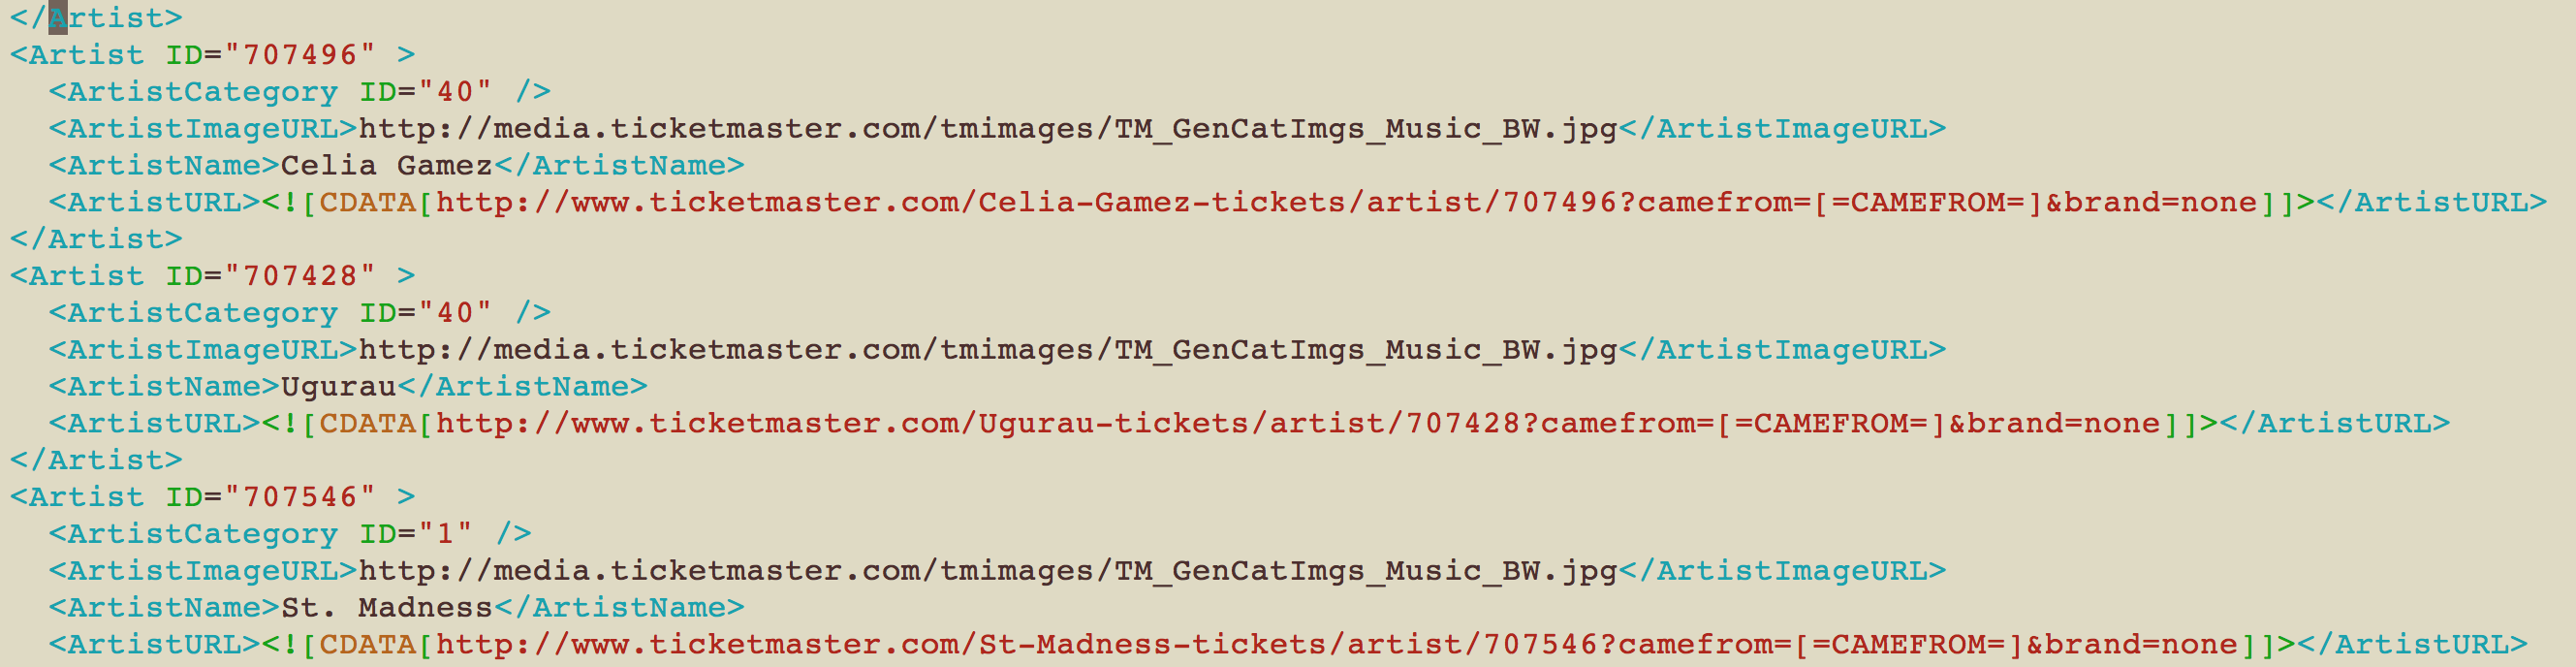
\includegraphics[width=90mm]{./pics/xml1.png}
		       		\captionof{figure}{XML data schema}
		       	\end{center}
		       	For each artist, Ticketmaster has provided us the artist id, the category to which this artists 
		       	belongs, an url to the artist’s image (low resolution), the artist name, and an url to the artist page 
		       	on ticketmaster’s website.
		       	
		       	For each venue, Ticketmaster has provided us the city of the venue, the state of the venue, the 
		       	street of the venue, an url to the venue’s image, the name of the venue, an url to the venue’s page 
		       	on ticketmaster’s website and the zip code of the venue.
		       	
		       	For each event, Ticketmaster has provided us the event id, the performer ids (artist ids), the 
		       	category id of the event, the event date, event status, event time, on sale date, performance name, 
		       	the url to the ticketmaster page, and the venue id.
		       	
		       	\paragraph{Affinity Data Feed}
		       	The affinity data provided by Ticketmaster is a 11.1MB text file. The file contains an entry for 
		       	artists. Each artist’s entry has a list of scores and corresponding artists. The artists under an entry 
		       	are the recommended artists for the artist in question and each recommended artist is associated 
		       	with a score ranging from 0 - 1.
		       	\begin{center}
		       		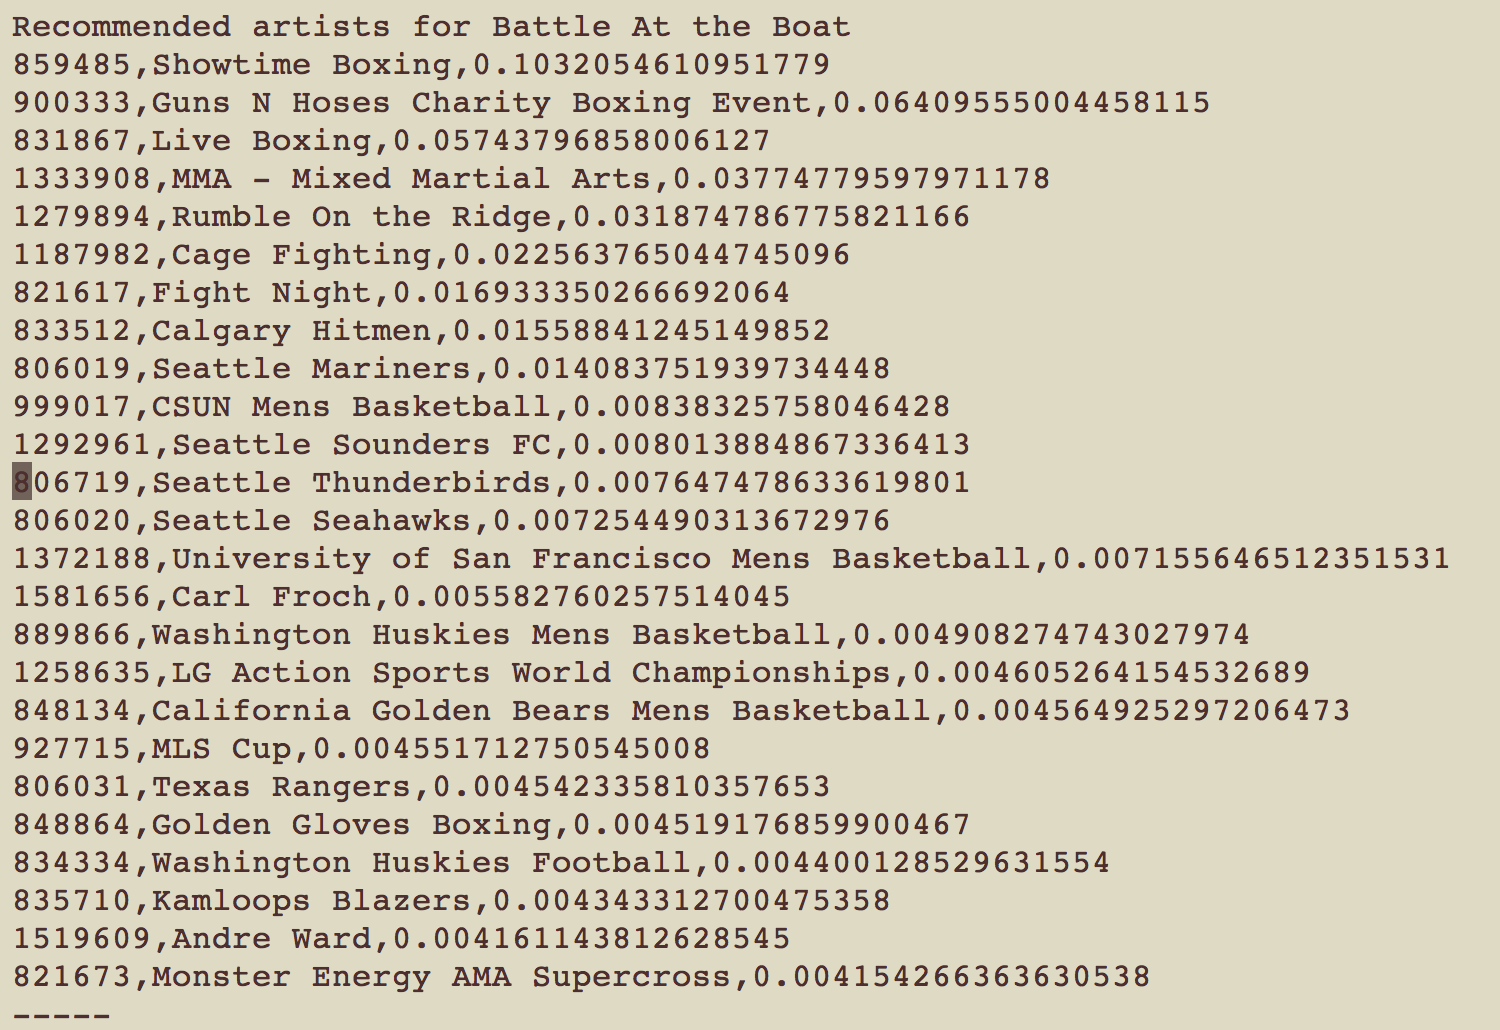
\includegraphics[width=90mm]{./pics/txt1.png}
		       		\captionof{figure}{Recommendation data form}
		       	\end{center}
		       	The format of the file is
		       	\begin{center}
		       	\textit{ArtistName} \\
		       	\{\textit{RecArtistID, RecArtistName, Score}\} *
		       	 \end{center}
		       	 "RecArtistID" can be related to the artist information in the event info data feed we have. The 
		       	 second value is the name of the recommended artist. The third value is the score ranging from 
		       	 0-1, with higher score meaning that the recommended artist is a better match than other artists 
		       	 with lower scores. This file is parsed using our custom Python script and stored on Parse.
		    \subsubsection{ Assumptions and Dependencies}
		     The major dependency for Tickets Tonight is its reliance on Parse. Tickets Tonight queries the data 
		     on Parse in order to generate its feed and explore views. If Parse cannot provide reliable service then 
		     the application interface with Parse will have to be changed and another form of data interface would 
		     be needed. 
	   